\section{\gls{mtbusb} v4}

\begin{figure}[ht]
%\includegraphics[width=0.7\textwidth]{data/mtb-topology.pdf}
\caption{Prototyp modulu MTB-USB.}
\label{fig:mtbusb-prototype}
\end{figure}

\gls{mtbusb} modul vzniknuvší v rámci této práce byl navržen kompletně nový,
inspirace starým \gls{mtbusb} modulem je minimální. Vznikly hardware, firmware
a popisy komunikačních protokolů.

Hlavním úkolem \gls{mtbusb} modulu je přeposílat data mezi sběrnici \gls{mtbbus}
a počítačem. \gls{mtbusb} modul provádí časově kritické operace sběrnice
 – například počítání timeoutu odpovědi na zprávu od \gls{mtb} modulů; pravidelné
dotazování \gls{mtb} modulů. Počítač pak informuje formou událostí.

\subsection{Komunikační protokol s počítačem}

Před návrhem samotné implementace je třeba navrhnout komunikační protokol
s počítačem. Tento komunikační protokol musí být přirozeně jiný, než nový
komunikační protokol sběrnice \gls{mtbbus}, který jsme popsali v předchozí
kapitole, protože zahrnuje jiné aktéry a funguje na jiné hardwarové platformě.

Komunikační protokol \gls{mtbusb} desky a počítače je navržen tak, aby byl do
velké míry nezávislý na protokolu sběrnice \gls{mtbbus}. Zásadním příkazem
je příkaz na přeposlání zprávy mezi \gls{usb} a \gls{mtbbus}. Tento příkaz umožňuje
počítačovému programu přeposlat libovolnou zprávu pro libovolný \gls{mtb} modul
(a naopak), aniž by \gls{mtbusb} deska musela znát sémantiku příkazů sběrnice
\gls{mtbbus}. Protokol sběrnice \gls{mtbbus} byl vytvářen přesně s tímto
cílem.

Na \gls{mtbusb} desku můžeme tedy pohlížet v zásadě jako na tenkého
přeposílatele mezi dvěma různými sběrnicemi – tzv. \textit{gateway}.

Plnohodnotná specifikace protokolu mezi počítačem a \gls{mtbusb} deskou je
k disopzici na \url{https://github.com/kmzbrnoI/mtbbus-protocol/tree/master/pc}.
Popišme nyní stručně návrh protokolu.

Mezi počítačem a \gls{mtbusb} deskou se komunikuje po virtuálním sériovém portu
(tzv. \textit{\gls{cdc}}) tunelovaným skrze \gls{usb} rozhraní. Toto řešení bylo vybráno,
protože je prakticky standardem pro připojením speciálních periferií k počítači.
Zvažován byl také například \textit{HID}. Samotná sběrnice \gls{usb}
nepodoporuje pojem zprávy tak, jak bychom ho vyžadovali\footnote{Při užití třídy \gls{cdc}
se data posílají nejčastěji každou milisekundu a to v bloku o nejvýše 64 bytech.
Počítačová aplikace díky bufferování operačního systému není schopna tyto bloky
spolehlivě rozlišit.}. Protože USB podporuje pouze 8bitový sériový port, začátek
zprávy je třeba označit jiným způsobem. v navrhovaném protokolu je začátek zprávy
označen speciální sekvencí dvou bytů \texttt{0x2A 0x42}. Tato sekvence se sice
ve zprávě může objevit, ale pravděpodobnost, že dojde k tolika chybám, aby
tato sekvence uprostřed zprávy byla považovaná za začátek zprávy, je
malá.\footnote{Uvědomme si, že rozdělování dat do zpráv na straně přijímače
se nemusí řídit jen detekcím magické sekvence bytů. Pokud zprávy nechodí moc
často, lze po delší době nepřijímání dat (třeba jednotky milisekund) vyprázdnit
vstupní buffer a očekávat, že další příchozivší data budou novou zprávou. Odesílací
strana nesmí odesílat jednotlivé části zprávy s velkou prodlevou, to je ale
rozumný požadavek.}

Celková struktura zprávy vypadá následovně (op jednotlivých bytech):

\begin{compactenum}
\item \texttt{0x2A},
\item \texttt{0x42},
\item počet následujících bytů,
\item kód příkazu,
\item data (až 122 bytů).
\end{compactenum}

Struktura je podobná struktuře zprávy protokolu \gls{mtbbus}, viz
\ref{subsub:mtbbus-proto-strucure}. Pozorný čtenář si přesto všimne například
chybějícího kontrolní součtu. Ten chybí, protože integritu zprávy řeší přímo
sběrnice \gls{usb} a tak ji není třeba řešit znovu. Upozorňujeme, že
\textit{kód příkazu} není kód příkazu sběrnice \gls{mtbbus}, ale kód příkazu
protokolu PC – \gls{mtbusb}.

Zprávy od počítače pro \gls{mtbusb} modul jsou:

\begin{itemize}
\item \textbf{Forward packet to \gls{mtbbus}}

V \textit{datech} příkazu následuje příkaz pro \gls{mtb} modul a adresa modulu,
kterému má být příkaz poslán.

\item \textbf{MTB-USB Information Request}

\item \textbf{Change Speed}

Požadavek na změnu komunikační rychlosti \gls{mtbusb} modulu. Změnu rychlosti
jednotlivých \gls{mtb} modulů je třeba provést předchozím příkazem, typicky
broadcastem všem \gls{mtb} modulům.

\item \textbf{Active modules request}

Odopovědí na tento příkaz je seznam aktivních adres \gls{mtb} modulů.
\end{itemize}

Zprávy od \gls{mtbusb} desky pro počítač:

\begin{itemize}
\item \textbf{Acknowledgement}
\item \textbf{Error}
\item \textbf{Packet from \gls{mtbbus}}

Zpráva je odeslána počítači při odpovědi \gls{mtb} modulu na příkaz počítače
nebo na pravidelný sken \gls{mtb} modulů. Z pohledu počítače tak přichází jak
odpovědi na příkazy pro \gls{mtb} modul, které poslal počítač, tak asynchronní
události – například změna stavu vstupů.

\item \textbf{\gls{mtbusb} Information}

\item \textbf{Active modules list}

\item \textbf{New module discovered event}

\item \textbf{Module failed event}

\end{itemize}

\gls{mtbusb} deska si udržuje seznam aktivních adres sběrnice. \textit{Polling}
modulů probíhá v iteracích. V každé iteraci jsou osloveny všechny aktivní
moduly a 10 neaktivních modulů. Tím je zaručeno, že aktivní moduly jsou
skenovány často a zároveň jsou detekovány nové moduly.

Pokud \gls{mtb} modul neodpoví na \textit{Module Inquiry}
(\ref{subsub:mtbbus-messages}), počítači je odeslána zpráva \textit{Module
failed event}. Modul je považován za ztracený, jakmile neodpoví na výzvu
ve třech po sobě jdoucích iteracích. Zpráva \textit{Module failed event}
je tedy při výpadku modulu odeslána třikrát. Zpráva obsahuje počet zbývajících
pokusů. Zpráva počítači o neodpovězení modulu je odeslána při každém neodpovězení,
nikoliv až při finálním označení modulu za neaktivní, aby bylo možné z počítače
monitorovat chod sběrnice. Občasné neodpovídání modulů na výzvy je dobrým
indikátorem problémů se sběrnicí.

Vlastností \gls{mtbbus} protokolu je, že každý \gls{mtb} modul musí vždy
odpovědět na každou zprávu, kterou dostane\footnote{Výjimkou jsou pouze
\textit{broadcast} zprávy.}. Protože \gls{mtbbus} je potenciálně nespolehlivé
médium, na kterém integritu příkazů kontrolujeme vlastními mechanismy, provádí
modul \gls{mtbusb} retransmisi zpráv pro \gls{mtb} moduly v případě, že na zprávy
nepřijde žádná odpověď, a to až třikrát. Proto součástí zprávy \textit{Packet
from \gls{mtbbus}} je také počítadlo, které říká, na kolikátý pokus byla tato
odpověď přijata (u asynchronních událostí 0). Toto číslo bylo do protokolu
vloženo opět se záměrem, aby bylo možné v počítači monitorovat chod sběrnice.

Na dalších příkazech protokolu není vcelku nic zajímavého, pokud je čtenář chce
prostudovat, je mu k dispozici plná specifikace protokolu na
\url{https://github.com/kmzbrnoI/mtbbus-protocol/tree/master/pc}.

TODO příklad skutečných dat?

\subsection{Hardware}

Srdcem desky je procesor \texttt{STM21F103}. Jedná se o moderní mikrokontrolér
rodiny \textit{ARM}, který autor zvolil z několika důvodů.

\begin{compactenum}
\item Procesor \texttt{STM32F103} má hardwarovou podporu \gls{usb}.
\item Procesory \texttt{STM32} nabízí velké velikosti pamětí a výpočetní výkon.
\item Procesory \texttt{STM32} se stávají standardy ve vestavěných systémech.
\item Procesory \texttt{STM32} se dají velice snadno debugovat.
\item Procesor \texttt{STM32F103} je jako jeden z mála \texttt{STM} součástí
	\textit{basic} součástek na \url{https://jlcpcb.com/}.
\item Autor se chtěl naučit pracovat s novou architekturou procesorů.
\end{compactenum}

Zastavme se krátce u některých bodů.

Hardwarová podpora \gls{usb} umožňuje výrazně vyšší flexibilitu komunikace
práce s počítačem, než použití historicky zaužívaných převodních obvodů mezi
\gls{usb} a sériovou linkou procesoru. V programu procesoru je tak například
možné definovat, že procesor má více \gls{cdc} linek – druhá se hodí například
pro ladění programu. Procesor může používat libovolnou třídu \gls{usb}. Celé
řešení se tak stává mnohem lépe upravitelné pouze změnou softwaru, což je
zásadně méně pracné, než změna hardwaru.

Všechny desky plošných spojů navrhnuté v rámci této práce, jsou navrženy tak,
aby se daly automaticky osazovat na \url{https://jlcpcb.com/}\footnote{Aktuálně
lze osazovat pouze jednu stranu desky a pouze \textit{SMD} součástky.}. Tato
firma nabízí velice levné automatické osazování malých sérií desek, což výrazně
zjednodušuje nasazení nových desek plošných spojů. JLCPCB rozlišuje tzv.
\textit{basic} a \textit{extended} součástky k osazení, přičemž za
\textit{basic} se neplatí režijní poplatek při osazování. \textit{basic}
součástky jsou ty, které se používají skutečně často (typicky diskrétní
součástky – rezistory, kondenzátory apod.) a které se budou vyrábět i za
desítky let.

Schéma a výkres desky plošných spojů byly vytvořeny v nástroji \textit{KiCad},
který autor této práce používal poprvé. Jedním z hlavních přínosů celé této
práce pro něj je, že se naučil pracovat s novými nástroji. Schéma a výkres
desky plošných spojů jsou k dispozici
online\footnote{\url{https://github.com/kmzbrnoI/mtb-usb-4-pcb}}, schéma je
přiloženo jako příloha této práce (\ref{aa}).

Popišme nyní stručné schéma. Na první pohled je schéma rozděleno na 2 části,
které jsou na desce plošných spojů (\textit{\gls{dps}}) galvanicky oddělené –
\gls{usb} část (vlevo) a \gls{mtbbus} část (vpravo). \gls{usb} část obsahuje
procesor a je napájena přímo z \gls{usb}. \gls{mtbbus} část obsahuje rozhraní
sběrnice \gls{mtbbus} a je napájeno buď z externího zdroje (ze stejného jako
zbytek sběrnice \gls{mtbbus}) nebo přes galvanicky oddělený měnič \texttt{PS1}.
Při osazení desky se osazením nebo neosazením součástek zvolí, která varianta
se bude používat.

Hlavním prvkem \gls{usb} části schématu je již zmíněný procesor
\texttt{STM32F03} (vlevo nahoře). K procesoru jsou připojena diagnostická
rozhraní (\texttt{J2}, \texttt{J3}). Celá \gls{usb} část na napájena z \gls{usb}
portu, přičemž je využito moderního konektoru \gls{usb}-C.

Rozhraní \gls{usb} a \gls{mtbbus} části schématu tvoří galvanicky oddělený
driver sběrnice RS485 typu \texttt{ADM2483}. Jedná se o osvědčený driver,
který zvládá proudy sběrnice až do $200~mA$ \cite{adm2483-datasheet} a je tedy
vhodný pro komunikaci s větším počtem \gls{mtb} modulů.

Specialitou \gls{mtbusb} modulu je měřící obvod \texttt{INA219}, který měří
napětí a proud do sběrnicové části obvodu \texttt{ADM2483} a posílá naměřenou
hodnotu do procesoru (skrze galvanické oddělení sběrnice \textit{I2C}). Počítač
je tak schopen detekovat nestandardní chování sběrnice, například zkrat.
\footnote{Pro tento hardware zatím neí podpora v komunikačním protokolu
s~počítačem a ve firmwaru. Hardware je odzkoušený. Podporu je v~plánu doplnit
v~další verzi.}

Při návrhu desky plošných spojů bylo hlavním problémem do jaké krabičky desku
vložit. \gls{mtbusb} modul totiž typicky není pevnou součástí kolejiště, je
umístěn vedle kolejiště u řídicího serveru. Vyvstal tak požadavek modul zavřít
do krabičky, ideálně s možností uchycení na zeď. Po rešerši byla zvolena krabička
firmy \textit{Digikeijs}, jejíž zásadní výhodou je to, že pro vyvedení konektorů
a indikačních LED není třeba do krabičky frézovat. Navíc lze na krabičku velice
elegantně nalepit potisk, který vysvětluje použití jednotlivých konektorů
a~význam LED. Celé řešení je zobrazeno na úvodním obrázku
\ref{fig:mtbusb-prototype}.


\subsection{Firmware}

Firmware je psaný v jazyce C, který byl zvolen především proto, že ve stejném
jazyce je psána základní knihovna pro interakci s periferiemi procesoru
\textit{STM32 HAL} \cite{stm32-hal}, kterou firmware využívá.

Při práci s periferiemi je využito \textit{Direct Memory Access (DMA)}. Pro
komunikaci přes \gls{usb} byla využita komunitní knihovna \texttt{libusb\_stm32},
\footnote{\url{https://github.com/dmitrystu/libusb_stm32}}.

Celý firmware je k dispozici pod opensource licencí na
\url{https://github.com/kmzbrnoI/mtb-usb-4-fw}.


\section{\gls{mtbuni} v4}

Další komponentou nového systému \gls{mtb} je nový modul typu \gls{mtbuni}.

\subsection{Základní parametry modulu}

\begin{table}[h]
	\begin{tabularx}{\textwidth}{lX}
		\toprule
		Vstupy & 16 digitálních vstupů \\
		Výstupy & 16 výstupů v režimu otevřeného kolektoru, všechny umožňují
		kmitání a generování S-COM signálu \\
		Napájení & 7–17 V DC \\
		Adresování & pomocí jumperů \\
		Procesor & ATmega128 \\
		\bottomrule
	\end{tabularx}
	\caption{Základní parametry modulu \gls{mtbuni} v4}
	\label{tab:mtbuni-params}
\end{table}

Aktuální modul \gls{mtbuni} má 16 digitálních vstupů a 16 digitálních výstupů.
Tento počet se autor práce rozhodl zachovat, protože vhodně škáluje pro malé
i~velké stanice. Současné \gls{mtbuni} a MTB-TTL desky používají různé konektory
pro připojení periferií: svorkovnice nebo nasouvací konektory typu \texttt{PSH}
\footnote(Např. \url{https://www.gme.cz/konektor-se-zamkem-psh02-04pg}.).
Modul \gls{mtbuni} v4 umožňuje variantní osazení jak svorkovnic, tak konektorů
\texttt{PSH}. Tím modul slučuje současné moduly \gls{mtbuni} a MTB-TTL do jediné
desky plošných spojů, což zjednodušuje údržbu a vývoj.

Hardwarové řešení výstupů je ponecháno: výstupy jsou v režimu otevřených
kolektorů. Výstupy jsou řízení skrze obvody \texttt{ULN2803}, které umožňují
dostatečný výstupní proud až 0.5~A~/~8 výstupů. Všechny výstupy umožní kmitání
i zasílání signálu S-COM \ref{scom}.

Modul obsahuje 16 digitálních vstupů. Podporu IR čidel bude řešit samostatná
deska, viz \ref{}.

Deska plošných spojů je navrhnuta tak, aby byly zachovány rozměry a umístění
upevňovacích otvorů se současným nejmenším modulem – MTB-TTL.

Návrh této desky vznikal ve spolupráci s \textit{Mendelovou univerzitou v Brně},
schéma vytvořil Robert Čížek, deska plošných spojů, firmware a koncepční návrh
modulu je dílem autora této práce.


\subsection{Hardware}

Při návrhu modulu připadaly v úvahu dva zásadní přístupy:

\begin{compactenum}
\item malý proces, posuvné registry na vstupy a výstupy;
\item velký procesor, vstupy a výstupy připojené přímo na piny procesoru.
\end{compactenum}

Autor této práce zvolil přístup (2), protože chtěl minimalizovat počet
součástek na desce a protože v dnešní době není problém sehnat fyzicky malý
procesor s~40 piny.

Schéma i deska plošných spojů jsou openhardware projekt, dostupné na
\url{https://github.com/kmzbrnoI/mtb-uni-4-ele}, schéma také v příloze
\ref{}. Zmiňme nyní zajímavé prvky schématu a desky plošných spojů.

Jádrem desky je procesor \texttt{ATmega128A}. Autor této práce si zvolil
procesor architektury \textit{AVR}, protože s používáním těchto procesorů má
dlouholeté zkušenosti. Model \textit{ATmge128a} byl pak zvolen proto, že je to
nejmenší model rodiny \textit{ATmega}, který obsahuje požadované množství pinů.

\subsubsection{Vstupy}

Nový \gls{mtbuni} v4 modul oproti modulu současnému obsahuje řádnou ochranu
vstupů. Ochranný obvod vstupů vznikl ve spolupráci Jana Horáčka, Michala
Petrilaka a Roberta Čížka. Zapojení jednoho vstupu je demonstrováno na obrázku
\ref{fig:mtbuni-input}.

\begin{figure}[ht]
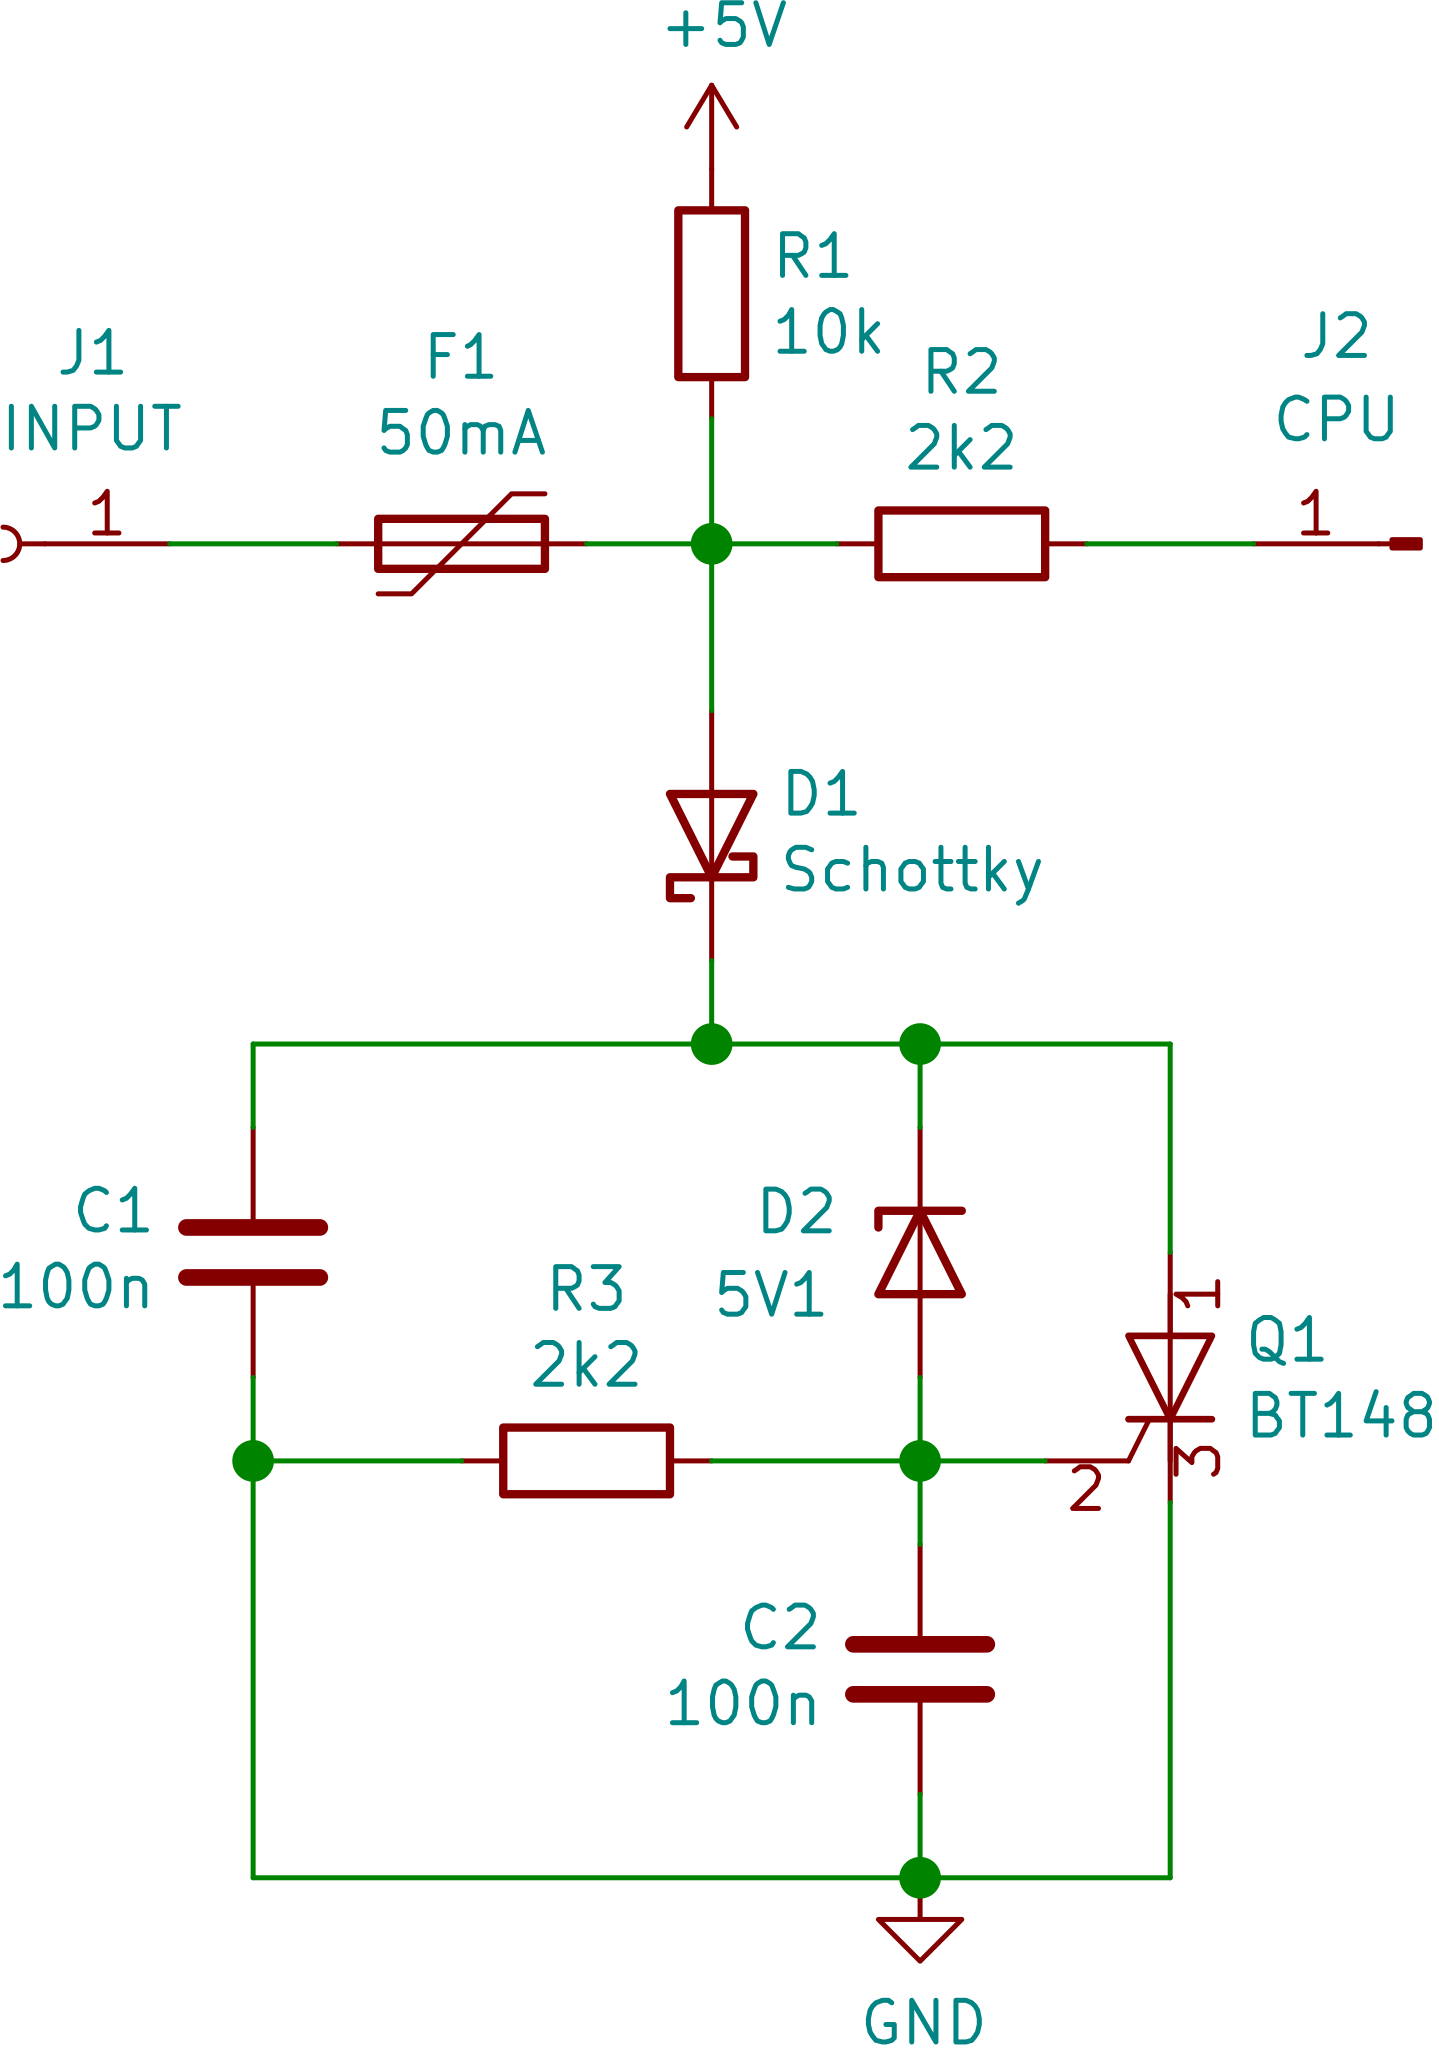
\includegraphics[width=0.4\textwidth]{data/uni-input/uni-input.pdf}
\caption{Zapojení vstupu modulu MTB-UNI.}
\label{fig:mtbuni-input}
\end{figure}

Schéma \ref{fig:mtbuni-input} je rozděleno na 2 části schottkyho diodou
\texttt{D1}. Horní část včetně diody \texttt{D1} je pro každý z 16 vstupních
pinů zvlášť, spodní je vždy pro osmici pinů společná.

Očekává se, že periferie připojená k pinu (\texttt{INPUT}) bude tento pin
uzemňovat, případně že bude pin v režimu \gls{ttl}. Každý vstup obsahuje
pull-up rezistor \texttt{R1}, aby měl vstupní signál vždy definovanou napěťovou
úroveň. Pull-up rezistor je relativně tvrdý, aby se zabránilo ovlivňování
vstupů okolním rušením, které signál \gls{dcc} při přenášení větších proudů
bohužel generuje.

K procesoru vede signál přes ochrannou pojistku \texttt{F1} (význam vysvětlíme
niže) a ochranný rezistor \texttt{R2}. Tento rezistor zabraňuje naproudu do pinu
procesoru a tím jeho zničení.

Funkcí celého obvodu od \texttt{D1} níže je vyzkratovat vstup na zem v momentě,
kdy je na něj přivedené vyšší než dovolené napětí. Pin procesoru povoluje
napětí nejvýše $5.5~V$ \cite{atmega128-datasheet}. Jakmile se vstupní napětí
začne blížit $5.4~V$ ($5.1~V$ zenerova dioda \texttt{D2} + $0.3~V$ schottkyho
dioda \texttt{D1}), začne se dioda \texttt{D2} otevírat a tím se začne otevírat
i tyristor \texttt{Q1}.\footnote{V praxi tato situace nastává už při trochu
nižším napětí, cca $5.3~V$, protože pro otevření \texttt{Q1} stačí, aby se
\texttt{D2} otevřela jen nepatrně.} Vstupní proud proteče přes \texttt{Q1} do
země a tím je vstup zkratován (do země). Proud je limitován pojistkou \texttt{F1}.
Tyristor \texttt{Q1} dimenzován jako výkonový, protože do něj může téct zkratový
proud všemi 8 piny, navíc chování polymerové pojistky umožňuje krátkodobé řádově
větší proudy, které musí tyristor zvládnout \cite{polyfuse-behavior}.

V praxi se často používá zapojení \textit{vstup – ochranný rezistor – pull-up –
pin procesoru}. V zapojení \gls{mtbuni} desky za oproti tomu používá zapojení
\textit{vstup – pull-up – ochranný rezistor – pin procesoru}. Výhodou zapojení,
které bylo implementováno do \gls{mtbuni} modulu, je, že na vstupu procesoru
není napěťový dělič. V případě, že vstup má například napětí $0.7~V$ (což se
snadno stane například tehdy, když periferie používá výstupy typu otevřené
kolektory), je toto napětí přivedeno přímo na pin procesoru a tedy spolehlivě
detekováno jako logická nula\footnote{V~\gls{mtbuni} desce je detekováno
jako logická jednička, protože modul používá inverzní logiku.}. Při zapojení
prvního typu by na pinu procesoru vznikl napěťový dělič, který by mohl ohrozit
spolehlivost čtení pinu.

\subsubsection{Výstupy}

Na výstupech je použito již zmiňovaných obvodů \texttt{ULN2803}. Za obvody
je vřazena polymerová pojistka. Protože obvod \texttt{ULN2803} specifikuje
proudové omezení $0.5~A$ / všechny výstupy \cite{uln2803-datasheet}, nemohou
samostatné pojistky zajistit nepřetížení modulu a zároveň umožnit využití
maximálního proudu. Proto jsou na desce plošných spojů \gls{mtbuni} v4 obvody
\texttt{ULN2803} jako jedny z mála osazeny v paticích v \textit{DIL} provedení.

Výstupy obsahují ochranu proti přivedení vysokého napětí, kterou realizuje
stejný obvod, jako na obrázku \ref{fig:mtbuni-input} (obvod pod diodou
\texttt{D1}). Obdobný obvod realizuje ochranu také proti vysokému napájecímu
napětí celého modulu. Viz kompletní schéma \ref{mtbuni-sch}.

\subsubsection{Adresování}

Adresa modulu \gls{mtbuni} v4 je určena jumpery na modulu. Při návrhu modulu
vyvstala diskuze, jaký je nejlepší způsob adresování modulů, přičemž soupeřily
přístupy

\begin{compactenum}
\item modul má adresu uloženou v EEPROM, adresu je možné změnit přes \gls{mtbbus}
\item adresa se konfiguruje přímo jumpery na modulu.
\end{compactenum}

Druhý přístup, který zvolil autor této práce, si vysloužil mnohou kritiku.
Autor si však stojí za tím, že snadná a především vždy pravdivá identifikace
adresy modulu prostým pohledem na něj stojí za 8 vstupních pinů procesoru navíc.

Pro elegantní řešení přístupu (1) je třeba mít na desce tlačítko. Tlačítko se
na desce nachází, takže pokud by byla v budoucnu snaha přejít na přístup (1),
je změna otázkou změny firmwaru.

\subsection{Deska plošných spojů}

Deska plošných spojů je navrhnuta tak, aby byly zachovány rozměry a umístění
upevňovacích otvorů se současným nejmenším modulem – MTB-TTL. Deska je dvouvrstvá
(protože to stačí), používají se primárně SMD součástky velikosti 0805 umístěné
na spodní stranu desky (aby šla \gls{dps} automaticky osazovat). Na obrázku
\ref{dig:mtb-uni-v4} je prototyp desky \gls{mtbuni} v4.0. Poslední verze je
verze 4.2, která oproti 4.0 obsahuje více \textit{SMD} součástek a opravuje
některé chyby prototypu.

\begin{figure}[ht]
%\includegraphics[width=0.7\textwidth]{data/mtb-topology.pdf}
\caption{\gls{mtbuni} v4.0.}
\label{fig:mtb-uni-v4}
\end{figure}

\subsection{Firmware}

Firmware pro procesor \textit{ATmega128A} je psán v jazyce C a je dostupný
pod opensource licencí na \url{https://github.com/kmzbrnoI/mtb-uni-4-fw}.

Zajímavým prvkem firmwaru je podpora jeho aktualizace přímo přes sběrnici
\gls{mtbbus}. Firmware obsahuje 2 části:

\begin{compactenum}
\item hlavní program,
\item bootloader
\end{compactenum}

Bootloader je nahraný ve speciální části paměti (na konci) a zajišťuje
aktualizaci hlavního programu. Bootloader je měnitelný pouze přímým
programování procesoru, nikoliv přes \gls{mtbbus}. Firmware tak v zásadě
obsahuje 2 samostatné programy, které se po zkompilování slinkují dohromady.

Bootloader umí pouze aktualizovat firmware a kontrolovat jeho konzistenci.
Kontrola konzistence firmwaru je implementována pomocí uložení \textit{CRC-16}
kontrolního součtu a počtu aktivních stránek paměti na konkrétních adresách
paměti (na konci těsně před bootloaderem).

\section{MTB-2-AVR}


\section{IRdet}


\section{MTB daemon}


\section{hJOP MTB Network RCS knihovna}
